\begin{fullwidth}
\section{Conceptual Design}
This section of the design dossier captures the system design associated with the conceptual design. Specifically, it defines the subsystem function block and functional flows that help add details to the System Specification.

Additional project risk analysis is provided in the form of a feasibility analysis on select requirements and the provided Failure Mode, Effect and Criticality Analysis.

\subsection{Functional Block Diagram}
    The focus of this project is to create a fleshed-out concept of an AUAV with a unique set of highly technical capabilities. This section will provide a high-level description of the functional systems within the AUAV. The aim is to show the overall relationships of the system. The  high-level functional block diagram, shown in Figure \ref{}, has been included to illustrate the various functions that make up the AUAV. In order to achieve a successful mission, all these functions must cooperate to achieve their objective while interacting with all of the other functions in the AUAV. 

    \begin{figure}
        \centering
        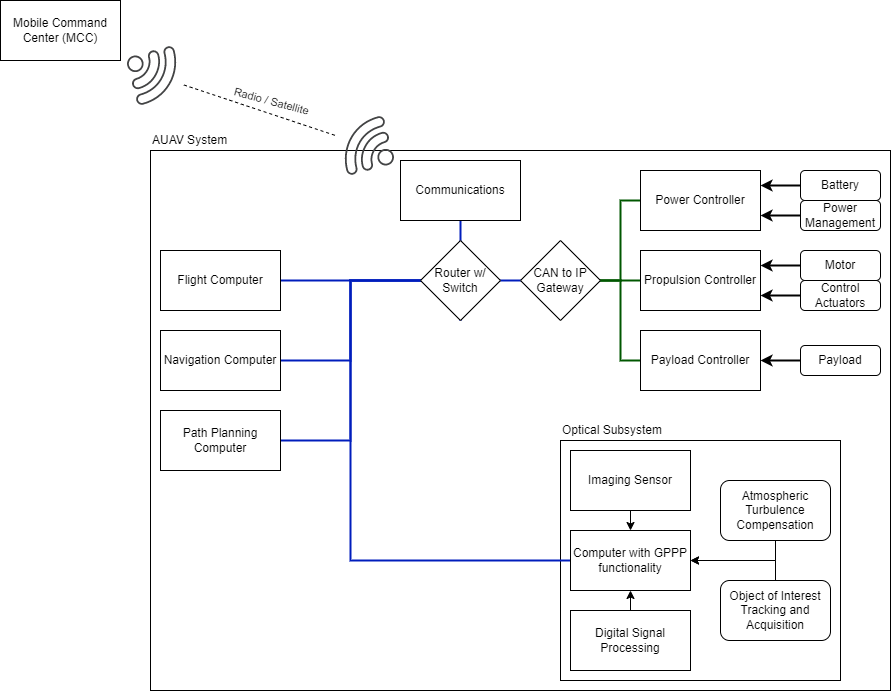
\includegraphics[height=6in]{01 - Design Dossier/images/UAV System Diagram-AUAV System.png}
        \caption{High Level System Functional Diagram}
        \label{fig:high_system_diagram}
    \end{figure}
\end{fullwidth}